\section{Per-pair Tables for Main-text Figures}
\label{app:main_tables}

This section provides the per-pair numerical breakdown for the lightweight clique ($\mathcal{C}_{\text{Light}}$) underlying the main-text figures (Figures~\ref{fig:small-bidir-ser}, \ref{fig:small-bidir-donor-util-id}, \ref{fig:small-bidir-base-util-slope}). All values are reported at the per-pair $\lambda$ from Appendix~\ref{app:lambda_sweep}; SER is measured on Alpaca, SQuAD v2, and GSM8K, and utility metrics follow the main-text choices (\S\ref{subsec:exp-settings}).

\subsection{Terminology and post-training regime}
\label{app:terminology}

We adopt \emph{base} (with \emph{recipient} as a synonym) and \emph{donor} as the names of the two models in the transplant. This naming follows the convention established by the dominant open-source tooling that motivated our threat model, \texttt{mergekit-tokensurgeon}~\citep{mergekit2024} and the training-free transplant operator of \citet{goddard2025tftransplant}, and is consistent with the broader vocabulary-adaptation literature that pairs ``donor''/``source'' with ``base''/``target''/``recipient'' interchangeably (e.g., \citep{minixhofer2021wechsel,dobler2023focus,ostendorff2023efficient}). The term \emph{base} as we use it carries \emph{no} commitment about whether the underlying checkpoint is purely pretrained or post-trained.

\noindent\textbf{Vendor naming for pretrained vs.\ instruction-tuned releases is not uniform.}
Some patterns are clear: \texttt{Qwen/Qwen2-0.5B} is a pretrained checkpoint and \texttt{Qwen/Qwen2.5-1.5B-Instruct} is its instruction-tuned variant; Gemma uses an explicit \texttt{-it} suffix; Ministral uses \texttt{-Instruct}; SmolLM2 uses \texttt{-Instruct}. Other vendors changed convention across releases: starting with the Qwen3 family, public releases such as \texttt{Qwen/Qwen3-0.6B} are post-trained by default, with pretrained-only variants now carrying a \texttt{-Base} suffix that we do not use here. Table~\ref{tab:model_aliases} lists every model identifier that appears in the paper.

Under these conventions, the purely pretrained models in our pool are the Qwen2 series (\texttt{Qwen2-0.5B}, \texttt{Qwen2-7B}), the Llama series (\texttt{Llama-3.2-1B}, \texttt{Llama-3.2-3B}, \texttt{Llama-3.1-8B}, \texttt{Meta-Llama-3-8B}), and \texttt{Mistral-7B-v0.1}. The remaining checkpoints (Qwen3 releases without \texttt{-Base}, all Gemma \texttt{-it} releases, \texttt{Ministral-3b-instruct}, \texttt{SmolLM2-1.7B-Instruct}, and \texttt{Qwen2.5-1.5B-Instruct}) are instruction-tuned.

\noindent\textbf{The pool covers all four base/donor cross-classifications.}
Because the experiments use exhaustive pairwise designs (lightweight and standard-scale cliques) and one-per-family cross-scale designs, the empirical evidence covers all four combinations of base and donor regime: pretrained$\to$pretrained, pretrained$\to$instruction-tuned, instruction-tuned$\to$pretrained, and instruction-tuned$\to$instruction-tuned. We treat this distribution as appropriate: a single experimental setting that mixes both regimes characterizes the construction's behavior across deployment settings, which a pretrained-only or IT-only pool cannot.

To avoid ambiguity from non-uniform vendor naming conventions, Table~\ref{tab:model_aliases} lists the pretrained/post-trained status of every checkpoint used in the paper. The per-pair tables below are color-coded by base/donor regime (\colorbox{rowPP}{\strut\,P$\to$P\,}, \colorbox{rowPI}{\strut\,P$\to$I\,}, \colorbox{rowIP}{\strut\,I$\to$P\,}, \colorbox{rowII}{\strut\,I$\to$I\,}; P: pretrained, I: instruction-tuned), making each experiment's regime composition explicit.

\subsection{Base-utility slope across attack stages and the $\lambda$-window}
\label{app:base_util_slope}
\label{app:lambda_window}

Figure~\ref{fig:small-bidir-base-util-slope} reports per-pair base-utility trajectories across the three model states (\emph{original} $\to$ \emph{after-OMP} $\to$ \emph{after-attack}) on Wikitext, LAMBADA, MMLU, and ARC-Challenge; each line is one (base$\leftarrow$donor) pair, with line color encoding the base model and marker shape the donor.

\noindent\textbf{$\lambda$-window ablation.} Figure~\ref{fig:ser-vs-hitsk} ablates the donor-suppression weight $\lambda$ on two pairs (Qwen3-1.7B$\leftarrow$Min-3B and Llama-3.2-1B$\leftarrow$Min-3B), tracking SER and Hits@$\{1,10,20\}$ on the Wikitext test set for both the base and the donor. Donor SER and Hits@1 collapse to near zero as $\lambda$ moves from $512$ to $768$, while attacked-base Hits@1 stays above $80\%$ even at $\lambda{=}2048$. The resulting wide operational window (e.g., $\lambda\in[768, 1536]$) does not require precise tuning, and matches the GSVD-spectral statement in Theorem~\ref{thm:wide-lambda-window} (Appendix~\ref{app:lambda-window}). $\lambda$ itself is selected on a held-out split of the WikiText corpus used to collect $\boldsymbol{\mu}_{\text{base}}$; this split is disjoint from the Alpaca / SQuAD~v2 / GSM8K prompt pools on which SER is evaluated, so $\lambda$ selection never touches the SER test data.

\begin{figure}[!htbp]
  \centering
  \begin{minipage}[t]{0.49\textwidth}
    \centering
    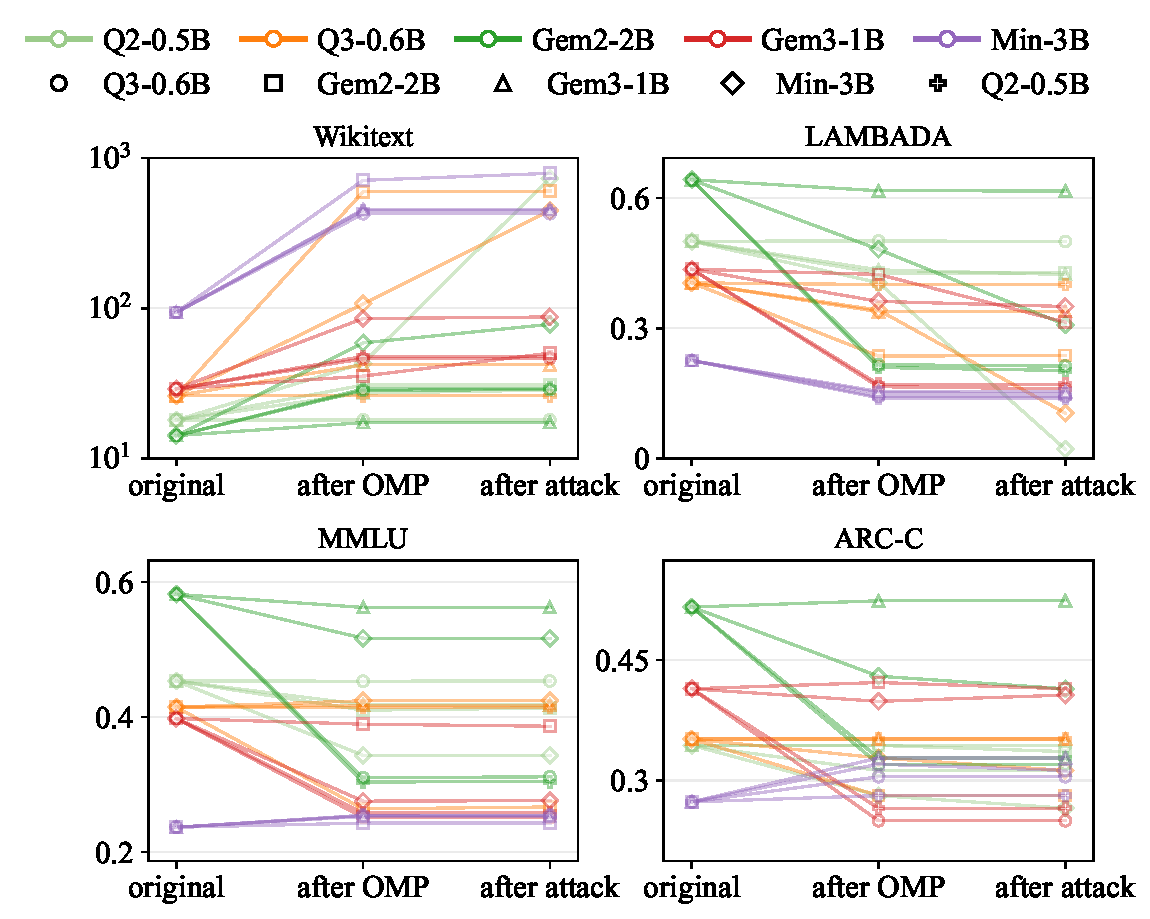
\includegraphics[width=\linewidth]{paper/figures/main_small_bidirectional_base_utility_slope_3stage.pdf}
    \captionof{figure}{\textbf{Three-stage base-utility slope charts.} Each line is one (base$\leftarrow$donor) pair: original $\to$ after-OMP $\to$ after-attack.}
    \label{fig:small-bidir-base-util-slope}
  \end{minipage}\hfill
  \begin{minipage}[t]{0.49\textwidth}
    \centering
    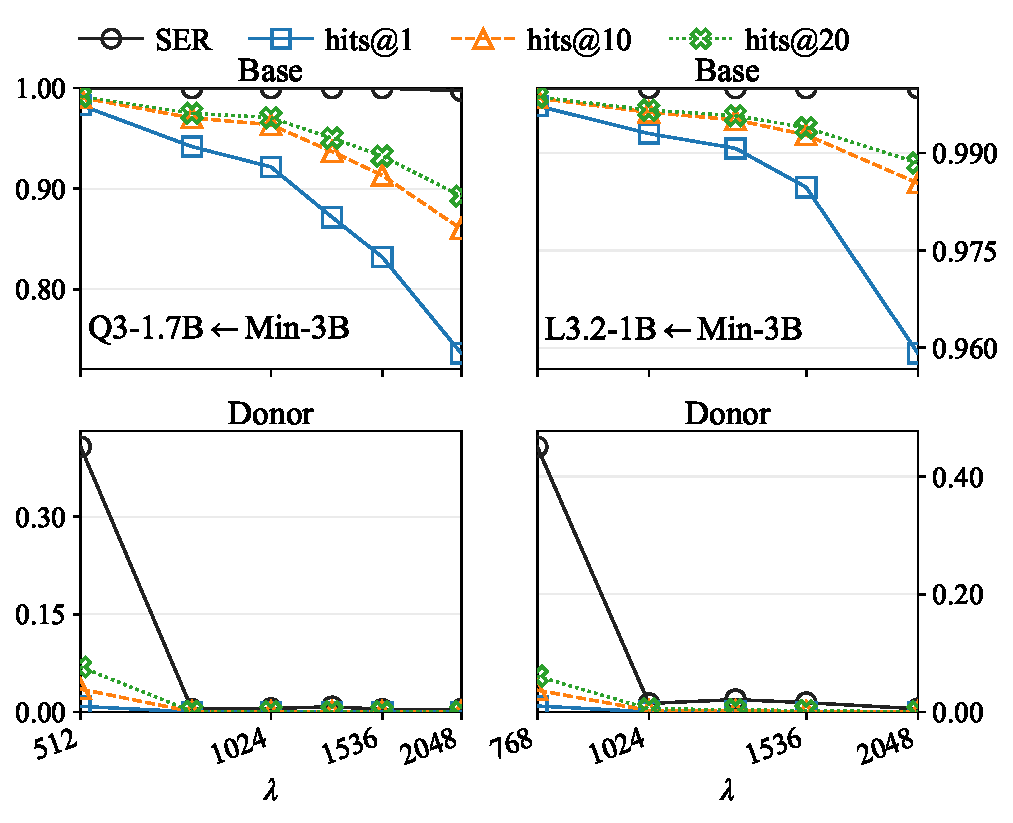
\includegraphics[width=\linewidth]{paper/figures/main_ser_vs_hitsk_varying_lambda.pdf}
    \captionof{figure}{\textbf{$\lambda$ creates a wide donor-suppression window.} Donor SER vanishes by $\lambda{=}768$ while attacked-base Hits@1 holds above $80\%$.}
    \label{fig:ser-vs-hitsk}
  \end{minipage}
\end{figure}

\subsection{Per-pair tables}
\label{app:main_tables_tables}

Each per-pool SER is estimated as a binomial proportion over $n{=}256$ prompts. For a proportion $\hat{p}$, the Wilson 95\% confidence interval is $[c(\hat{p})-\mathrm{hw}(\hat{p}),\, c(\hat{p})+\mathrm{hw}(\hat{p})]$, where $c(\hat{p})=(\hat{p}+z^{2}/(2n))/(1+z^{2}/n)$ and $\mathrm{hw}(\hat{p})=z\sqrt{\hat{p}(1-\hat{p})/n+z^{2}/(4n^{2})}/(1+z^{2}/n)$ with $z{=}1.96$. The single-value SER tables in the appendix (Table~\ref{tab:app:altops:ser} and Tables~\ref{tab:merge-mitigation-gem3}--\ref{tab:merge-mitigation-q2}) carry per-cell intervals in the form $\hat{p}\,_{[\mathrm{lo},\mathrm{hi}]}$; aggregate columns (Avg, $\mathrm{SER}_{\max}$) display the Wilson interval of the per-pool proportion that attains the reported value, not a strict interval for the aggregate functional. For the slash-pair per-pool tables we omit per-cell intervals to keep the table within page width; the same Wilson formula applies cell-by-cell.

\begingroup
\small
\setlength{\tabcolsep}{3pt}
\begin{longtable}{@{}llrrrrr@{}}
\caption{The Lightweight Clique ($\mathcal{C}_{\text{Light}}$) (per-pair SER; fractions)}\label{tab:app:small-bidirectional:ser}\\
\toprule
$B$ & $D$ & $\lambda$ & \multicolumn{4}{c}{SER (atk-base / pat-donor)} \\
\cmidrule(lr){4-7}
 &  &  & Alpaca & SQuAD & GSM8K & $\mathrm{SER}_{\max}$ \\
\midrule
\endfirsthead
\toprule
$B$ & $D$ & $\lambda$ & \multicolumn{4}{c}{SER (atk-base / pat-donor)} \\
\cmidrule(lr){4-7}
 &  &  & Alpaca & SQuAD & GSM8K & $\mathrm{SER}_{\max}$ \\
\midrule
\endhead
\bottomrule
\endfoot
\rowcolor{rowPI} Q2-0.5B & Q3-0.6B & 1280 & .0156/.0000 & .0156/.0000 & .0000/.0000 & .0156/.0000 \\
\rowcolor{rowPI} Q2-0.5B & Gem2-2B & 768 & .2266/.0430 & .2031/.0156 & .0234/.0117 & .2266/.0430 \\
\rowcolor{rowPI} Q2-0.5B & Gem3-1B & 512 & .6445/.0547 & .2930/.0781 & .1797/.0078 & .6445/.0781 \\
\rowcolor{rowPI} Q2-0.5B & Min-3B & 2048 & .9805/.0000 & .9844/.0039 & 1.0000/.0000 & 1.0000/.0039 \\
\rowcolor{rowIP} Q3-0.6B & Q2-0.5B & 1024 & .0000/.0000 & .0000/.0000 & .0000/.0000 & .0000/.0000 \\
\rowcolor{rowII} Q3-0.6B & Gem2-2B & 256 & .5742/.0000 & .6016/.0039 & .5781/.0000 & .6016/.0039 \\
\rowcolor{rowII} Q3-0.6B & Gem3-1B & 1024 & .0000/.0000 & .0000/.0000 & .0000/.0000 & .0000/.0000 \\
\rowcolor{rowII} Q3-0.6B & Min-3B & 2048 & .9961/.0000 & 1.0000/.0078 & 1.0000/.0039 & 1.0000/.0078 \\
\rowcolor{rowIP} Gem2-2B & Q2-0.5B & 256 & .1367/.0078 & .3672/.0000 & .7734/.0000 & .7734/.0078 \\
\rowcolor{rowII} Gem2-2B & Q3-0.6B & 128 & .1406/.0000 & .6367/.0000 & .8789/.0000 & .8789/.0000 \\
\rowcolor{rowII} Gem2-2B & Gem3-1B & 128 & .0117/.0078 & .0117/.0039 & .0000/.0000 & .0117/.0078 \\
\rowcolor{rowII} Gem2-2B & Min-3B & 512 & .9922/.0078 & 1.0000/.0078 & .9844/.0000 & 1.0000/.0078 \\
\rowcolor{rowIP} Gem3-1B & Q2-0.5B & 512 & .0742/.0000 & .0859/.0039 & .3086/.0000 & .3086/.0039 \\
\rowcolor{rowII} Gem3-1B & Q3-0.6B & 512 & .3320/.0000 & .4727/.0000 & .6992/.0000 & .6992/.0000 \\
\rowcolor{rowII} Gem3-1B & Gem2-2B & 512 & 1.0000/.0000 & .9883/.0000 & 1.0000/.0000 & 1.0000/.0000 \\
\rowcolor{rowII} Gem3-1B & Min-3B & 2048 & .6562/.0078 & .7891/.0078 & .3398/.0000 & .7891/.0078 \\
\rowcolor{rowIP} Min-3B & Q2-0.5B & 1280 & .3125/.0117 & .2617/.0039 & .3906/.0000 & .3906/.0117 \\
\rowcolor{rowII} Min-3B & Q3-0.6B & 512 & .0547/.0000 & .0625/.0000 & .0898/.0000 & .0898/.0000 \\
\rowcolor{rowII} Min-3B & Gem2-2B & 256 & .9922/.0000 & 1.0000/.0000 & 1.0000/.0000 & 1.0000/.0000 \\
\rowcolor{rowII} Min-3B & Gem3-1B & 1024 & .1055/.0000 & .0977/.0000 & .1953/.0000 & .1953/.0000 \\
\end{longtable}
\endgroup

\begin{table}[t]
\centering
\caption{The Lightweight Clique ($\mathcal{C}_{\text{Light}}$) (base utilities; cells show pretrained/after-OMP/after-attack; value$\pm$stderr when available)}\label{tab:app:small-bidirectional:base-utils}
\resizebox{\linewidth}{!}{%
\begin{tabular}{@{}llrcccc@{}}
\toprule
&  &  & wikitext & lambada\_openai & mmlu & arc\_challenge \\
 $B$ & $D$ & $\lambda$ & word\_perplexity & acc & acc & acc\_norm \\
\midrule
\rowcolor{rowPI} Q2-0.5B & Q3-0.6B & 1280 & \ensuremath{18.02/18.04/18.05} & \ensuremath{.50\pm.01/.50\pm.01/.50\pm.01} & \ensuremath{.45\pm.01/.45\pm.01/.45\pm.01} & \ensuremath{.34\pm.04/.34\pm.04/.34\pm.04} \\
\rowcolor{rowPI} Q2-0.5B & Gem2-2B & 768 & \ensuremath{18.02/30.78/30.88} & \ensuremath{.50\pm.01/.43\pm.01/.43\pm.01} & \ensuremath{.45\pm.01/.41\pm.01/.41\pm.01} & \ensuremath{.34\pm.04/.34\pm.04/.34\pm.04} \\
\rowcolor{rowPI} Q2-0.5B & Gem3-1B & 512 & \ensuremath{18.02/27.24/28.53} & \ensuremath{.50\pm.01/.43\pm.01/.42\pm.01} & \ensuremath{.45\pm.01/.42\pm.01/.42\pm.01} & \ensuremath{.34\pm.04/.31\pm.04/.31\pm.04} \\
\rowcolor{rowPI} Q2-0.5B & Min-3B & 2048 & \ensuremath{18.02/43.02/734.85} & \ensuremath{.50\pm.01/.41\pm.01/.02\pm.00} & \ensuremath{.45\pm.01/.34\pm.01/.34\pm.01} & \ensuremath{.34\pm.04/.28\pm.04/.27\pm.04} \\
\rowcolor{rowIP} Q3-0.6B & Q2-0.5B & 1024 & \ensuremath{26.16/26.13/26.13} & \ensuremath{.40\pm.01/.40\pm.01/.40\pm.01} & \ensuremath{.41\pm.01/.41\pm.01/.41\pm.01} & \ensuremath{.35\pm.04/.35\pm.04/.35\pm.04} \\
\rowcolor{rowII} Q3-0.6B & Gem2-2B & 256 & \ensuremath{26.16/596.41/602.43} & \ensuremath{.40\pm.01/.24\pm.01/.24\pm.01} & \ensuremath{.41\pm.01/.26\pm.01/.27\pm.01} & \ensuremath{.35\pm.04/.28\pm.04/.28\pm.04} \\
\rowcolor{rowII} Q3-0.6B & Gem3-1B & 1024 & \ensuremath{26.16/42.04/42.02} & \ensuremath{.40\pm.01/.34\pm.01/.34\pm.01} & \ensuremath{.41\pm.01/.42\pm.01/.42\pm.01} & \ensuremath{.35\pm.04/.35\pm.04/.35\pm.04} \\
\rowcolor{rowII} Q3-0.6B & Min-3B & 2048 & \ensuremath{26.16/107.04/446.54} & \ensuremath{.40\pm.01/.34\pm.01/.10\pm.00} & \ensuremath{.41\pm.01/.42\pm.01/.42\pm.01} & \ensuremath{.35\pm.04/.33\pm.04/.31\pm.04} \\
\rowcolor{rowIP} Gem2-2B & Q2-0.5B & 256 & \ensuremath{14.19/28.95/29.39} & \ensuremath{.64\pm.01/.21\pm.01/.20\pm.01} & \ensuremath{.58\pm.01/.30\pm.01/.30\pm.01} & \ensuremath{.52\pm.04/.33\pm.04/.33\pm.04} \\
\rowcolor{rowII} Gem2-2B & Q3-0.6B & 128 & \ensuremath{14.19/28.40/28.79} & \ensuremath{.64\pm.01/.22\pm.01/.21\pm.01} & \ensuremath{.58\pm.01/.31\pm.01/.31\pm.01} & \ensuremath{.52\pm.04/.32\pm.04/.32\pm.04} \\
\rowcolor{rowII} Gem2-2B & Gem3-1B & 128 & \ensuremath{14.19/17.32/17.32} & \ensuremath{.64\pm.01/.62\pm.01/.62\pm.01} & \ensuremath{.58\pm.01/.56\pm.01/.56\pm.01} & \ensuremath{.52\pm.04/.52\pm.04/.52\pm.04} \\
\rowcolor{rowII} Gem2-2B & Min-3B & 512 & \ensuremath{14.19/58.79/78.11} & \ensuremath{.64\pm.01/.48\pm.01/.31\pm.01} & \ensuremath{.58\pm.01/.52\pm.01/.52\pm.01} & \ensuremath{.52\pm.04/.43\pm.04/.41\pm.04} \\
\rowcolor{rowIP} Gem3-1B & Q2-0.5B & 512 & \ensuremath{29.06/47.70/47.73} & \ensuremath{.44\pm.01/.17\pm.01/.17\pm.01} & \ensuremath{.40\pm.01/.26\pm.01/.26\pm.01} & \ensuremath{.41\pm.04/.27\pm.04/.27\pm.04} \\
\rowcolor{rowII} Gem3-1B & Q3-0.6B & 512 & \ensuremath{29.06/46.11/46.46} & \ensuremath{.44\pm.01/.17\pm.01/.16\pm.01} & \ensuremath{.40\pm.01/.25\pm.01/.25\pm.01} & \ensuremath{.41\pm.04/.25\pm.04/.25\pm.04} \\
\rowcolor{rowII} Gem3-1B & Gem2-2B & 512 & \ensuremath{29.06/35.35/50.24} & \ensuremath{.44\pm.01/.42\pm.01/.31\pm.01} & \ensuremath{.40\pm.01/.39\pm.01/.39\pm.01} & \ensuremath{.41\pm.04/.42\pm.04/.41\pm.04} \\
\rowcolor{rowII} Gem3-1B & Min-3B & 2048 & \ensuremath{29.06/85.42/87.50} & \ensuremath{.44\pm.01/.36\pm.01/.35\pm.01} & \ensuremath{.40\pm.01/.28\pm.01/.28\pm.01} & \ensuremath{.41\pm.04/.40\pm.04/.41\pm.04} \\
\rowcolor{rowIP} Min-3B & Q2-0.5B & 1280 & \ensuremath{93.86/446.98/447.70} & \ensuremath{.23\pm.01/.14\pm.00/.14\pm.00} & \ensuremath{.24\pm.01/.25\pm.01/.25\pm.01} & \ensuremath{.27\pm.04/.28\pm.04/.28\pm.04} \\
\rowcolor{rowII} Min-3B & Q3-0.6B & 512 & \ensuremath{93.86/425.86/426.14} & \ensuremath{.23\pm.01/.14\pm.00/.14\pm.00} & \ensuremath{.24\pm.01/.25\pm.01/.25\pm.01} & \ensuremath{.27\pm.04/.30\pm.04/.30\pm.04} \\
\rowcolor{rowII} Min-3B & Gem2-2B & 256 & \ensuremath{93.86/710.94/791.39} & \ensuremath{.23\pm.01/.15\pm.00/.15\pm.00} & \ensuremath{.24\pm.01/.24\pm.01/.24\pm.01} & \ensuremath{.27\pm.04/.32\pm.04/.31\pm.04} \\
\rowcolor{rowII} Min-3B & Gem3-1B & 1024 & \ensuremath{93.86/453.53/453.65} & \ensuremath{.23\pm.01/.15\pm.01/.15\pm.01} & \ensuremath{.24\pm.01/.25\pm.01/.25\pm.01} & \ensuremath{.27\pm.04/.33\pm.04/.33\pm.04} \\
\bottomrule
\end{tabular}}
\end{table}

\begingroup
\scriptsize
\setlength{\tabcolsep}{3pt}
\begin{longtable}{@{}llrcccc@{}}
\caption{The Lightweight Clique ($\mathcal{C}_{\text{Light}}$) (donor utilities; cells show pretrained/after-patch; value$\pm$stderr when available)}\label{tab:app:small-bidirectional:donor-utils}\\
\toprule
 &  &  & wikitext & lambada\_openai & mmlu & arc\_challenge \\
 $B$ & $D$ & $\lambda$ & word\_perplexity & acc & acc & acc\_norm \\
\midrule
\endfirsthead
\toprule
 &  &  & wikitext & lambada\_openai & mmlu & arc\_challenge \\
 $B$ & $D$ & $\lambda$ & word\_perplexity & acc & acc & acc\_norm \\
\midrule
\endhead
\bottomrule
\endfoot
\rowcolor{rowPI} Q2-0.5B & Q3-0.6B & 1280 & \ensuremath{26.16/26.14} & \ensuremath{.40\pm.01/.40\pm.01} & \ensuremath{.41\pm.01/.41\pm.01} & \ensuremath{.35\pm.04/.35\pm.04} \\
\rowcolor{rowPI} Q2-0.5B & Gem2-2B & 768 & \ensuremath{14.19/14.25} & \ensuremath{.64\pm.01/.64\pm.01} & \ensuremath{.58\pm.01/.58\pm.01} & \ensuremath{.52\pm.04/.52\pm.04} \\
\rowcolor{rowPI} Q2-0.5B & Gem3-1B & 512 & \ensuremath{29.06/29.96} & \ensuremath{.44\pm.01/.43\pm.01} & \ensuremath{.40\pm.01/.40\pm.01} & \ensuremath{.41\pm.04/.41\pm.04} \\
\rowcolor{rowPI} Q2-0.5B & Min-3B & 2048 & \ensuremath{93.86/93.90} & \ensuremath{.23\pm.01/.22\pm.01} & \ensuremath{.24\pm.01/.24\pm.01} & \ensuremath{.27\pm.04/.27\pm.04} \\
\rowcolor{rowIP} Q3-0.6B & Q2-0.5B & 1024 & \ensuremath{18.02/18.04} & \ensuremath{.50\pm.01/.50\pm.01} & \ensuremath{.45\pm.01/.45\pm.01} & \ensuremath{.34\pm.04/.34\pm.04} \\
\rowcolor{rowII} Q3-0.6B & Gem2-2B & 256 & \ensuremath{14.19/14.19} & \ensuremath{.64\pm.01/.64\pm.01} & \ensuremath{.58\pm.01/.58\pm.01} & \ensuremath{.52\pm.04/.52\pm.04} \\
\rowcolor{rowII} Q3-0.6B & Gem3-1B & 1024 & \ensuremath{29.06/29.06} & \ensuremath{.44\pm.01/.44\pm.01} & \ensuremath{.40\pm.01/.40\pm.01} & \ensuremath{.41\pm.04/.40\pm.04} \\
\rowcolor{rowII} Q3-0.6B & Min-3B & 2048 & \ensuremath{93.86/93.90} & \ensuremath{.23\pm.01/.22\pm.01} & \ensuremath{.24\pm.01/.24\pm.01} & \ensuremath{.27\pm.04/.27\pm.04} \\
\rowcolor{rowIP} Gem2-2B & Q2-0.5B & 256 & \ensuremath{18.02/18.04} & \ensuremath{.50\pm.01/.50\pm.01} & \ensuremath{.45\pm.01/.45\pm.01} & \ensuremath{.34\pm.04/.34\pm.04} \\
\rowcolor{rowII} Gem2-2B & Q3-0.6B & 128 & \ensuremath{26.16/26.14} & \ensuremath{.40\pm.01/.40\pm.01} & \ensuremath{.41\pm.01/.41\pm.01} & \ensuremath{.35\pm.04/.35\pm.04} \\
\rowcolor{rowII} Gem2-2B & Gem3-1B & 128 & \ensuremath{29.06/29.16} & \ensuremath{.44\pm.01/.44\pm.01} & \ensuremath{.40\pm.01/.40\pm.01} & \ensuremath{.41\pm.04/.40\pm.04} \\
\rowcolor{rowII} Gem2-2B & Min-3B & 512 & \ensuremath{93.86/93.90} & \ensuremath{.23\pm.01/.22\pm.01} & \ensuremath{.24\pm.01/.24\pm.01} & \ensuremath{.27\pm.04/.27\pm.04} \\
\rowcolor{rowIP} Gem3-1B & Q2-0.5B & 512 & \ensuremath{18.02/18.05} & \ensuremath{.50\pm.01/.50\pm.01} & \ensuremath{.45\pm.01/.45\pm.01} & \ensuremath{.34\pm.04/.34\pm.04} \\
\rowcolor{rowII} Gem3-1B & Q3-0.6B & 512 & \ensuremath{26.16/26.14} & \ensuremath{.40\pm.01/.40\pm.01} & \ensuremath{.41\pm.01/.41\pm.01} & \ensuremath{.35\pm.04/.35\pm.04} \\
\rowcolor{rowII} Gem3-1B & Gem2-2B & 512 & \ensuremath{14.19/14.19} & \ensuremath{.64\pm.01/.64\pm.01} & \ensuremath{.58\pm.01/.58\pm.01} & \ensuremath{.52\pm.04/.52\pm.04} \\
\rowcolor{rowII} Gem3-1B & Min-3B & 2048 & \ensuremath{93.86/93.90} & \ensuremath{.23\pm.01/.22\pm.01} & \ensuremath{.24\pm.01/.24\pm.01} & \ensuremath{.27\pm.04/.27\pm.04} \\
\rowcolor{rowIP} Min-3B & Q2-0.5B & 1280 & \ensuremath{18.02/18.05} & \ensuremath{.50\pm.01/.50\pm.01} & \ensuremath{.45\pm.01/.45\pm.01} & \ensuremath{.34\pm.04/.34\pm.04} \\
\rowcolor{rowII} Min-3B & Q3-0.6B & 512 & \ensuremath{26.16/26.14} & \ensuremath{.40\pm.01/.40\pm.01} & \ensuremath{.41\pm.01/.41\pm.01} & \ensuremath{.35\pm.04/.35\pm.04} \\
\rowcolor{rowII} Min-3B & Gem2-2B & 256 & \ensuremath{14.19/14.19} & \ensuremath{.64\pm.01/.64\pm.01} & \ensuremath{.58\pm.01/.58\pm.01} & \ensuremath{.52\pm.04/.52\pm.04} \\
\rowcolor{rowII} Min-3B & Gem3-1B & 1024 & \ensuremath{29.06/29.06} & \ensuremath{.44\pm.01/.44\pm.01} & \ensuremath{.40\pm.01/.40\pm.01} & \ensuremath{.41\pm.04/.42\pm.04} \\
\end{longtable}
\endgroup

